\chapter{iBeacon} \label{chap:ibeacons}
Apple introduced at its yearly Apple \ac{WWDC} 2013 a new technology, called \textit{iBeacon}, to enhance smartphone applications' location awareness.

An iBeacon, in general a beacon\footnote{\textit{iBeacon} is a registered trade mark of Apple}, is a System-on-Chip which emits a \textit{\ac{BLE}} signal in a predefined time interval, analogous to a lighthouse. % radio station
Devices with capable hardware and software, for example iPhone since iPhone 4S and Android since version 4.3, can receive the signals, to provide the user location based services.
Typically a beacon's size is less the size of a child's hand and is being powerd with a small battery to be independant of its environment.
Thus, it easily can be attached to another object to establish a region around the object.
A listening smartphone app can than show the user a notification when the user enterd or left a region, by estimating the proximity to the beacon \cite{apple:getting_started, binside:ds}.
Typical use-cases are \cite{binside:ds}:
\begin{itemize}
  \item Location based marketing (e.g.\ digital coupons, digital signage of articles)
  \item Proximity sensing to an object
  \item Indoor localization and navigation (e.g.\ digital museums guide, airport guide)
\end{itemize}

After providing a brief idea what a beacon actually is, we are going to focus in the next sections on the beacons itself and the communication technology which is being used by a beacon to send its signal.
Afterwards, we describe the \acs{API} provided by Apples mobile operating system iOS 8.1 to receive these signals.
After forming the foundation, we present our evaluation results of the received beacon signals on an iPhone 5S which are very important for the algorithm's implementation, described in chapter~\ref{chap:pf}.


\section{Bluetooth Low Energy}\label{sec:ble}
\ac{BT} is a wireless short range communication technology with the intend to replace resp.\ reduce the amount of necessary cables. The technologies key features are robustness, low cost and low power consumption.
It is often being used to connect a car's speaker phone with a smartphone, to connect a wireless keyboard or mouse with a computer, or to exchange files between two cell- or smartphones.
The \acl{BT} standard is being developed by the \emph{Bluetooth Special Interest Group (Bluetooth SIG)}, which is a large group of companies, that are interested in \acs{BT}.

Originally, the \acs{BT} specification contained just one wireless technology system called \emph{\ac{BR}/\ac{EDR}}.
Since version 4.0, released in 2010, the specification adds a second technology named \emph{\ac{LE}}.
Actually, the term \acs{LE} is just the technologies name inside of the specification but today it is also being used by the mainstream.
The technologies official (marketing) label is \emph{Bluetooth Smart}. Devices labeled with it are just equipped with the \acs{LE} technology.
Devices labled with \emph{Bluetooth Smart Ready} are equipped with both technologies, the traditional \acs{BR} and the \acs{LE} technology \cite{bluetooth:spec}.
One of the differences is the speed. \acs{BR}/\acs{EDR} has a max.\ transfer rate of 2-3~Mbps, \acs{LE} is just designed for 1~Mbps.
But, \acs{LE} has the advantage of having a low current consumption.
Its complexity is also lower than the one of \acs{BR}/\acs{EDR} \cite{bluetooth:spec}.

iBeacons usually are Bluetooth Smart, not Bluetooth Smart Ready devices \cite{binside:ds}.
To get a better idea of how the comunication between a smartphone and an iBeacon works, we give an overview of the \acs{BT} technology with focus on \acs{BLE}.
Both \acs{BT} systems are using the 2.4~GHz frequency band.


\paragraph{Channels and Events}
\acs{BLE} devides the band into 40 channels.
Three of them are advertisement channels, the others are data channels.
These channels are being used to send events.
An event consists of typical (data) packets that are being send over the channels.
The \acs{BLE} specification distinguishes between two events, the \emph{advertisment} and the \emph{connection} event.

Advertisement events are either being used for unidirectional or broadcast communication between two or more devices, or to establish a pair-wise or bidirectional communication.
This type of advertisment event is called a \emph{connectable advertisment}.
 Advertisment events are being send via one of the advertisment channels.
The device which sends the advertisement is called the \emph{advertiser}.
The device looking for these events is named \emph{scanner}.

If the device listens for a connectable advertisement it is called the \emph{initiator} and becomes the \emph{master} after establishing the connection.
The advertising device becomes the \emph{slave}.
Master and slave(s) are forming a piconet. Slaves in a piconet cannot communicate with each other.
The connection establishment takes place on one of the advertisement channels.
After establishing a connection, the communication takes place on the data channels by using frequency hopping instead of one specific channel \cite{bluetooth:spec}.

\paragraph{Operations}
\acs{BLE} implements different operations for the above mentioned event behaviour\cite{bluetooth:spec}.
\begin{itemize}
  \item To send advertisement events the \textbf{Advertismenet Procedure} is being used.
    It sends unidirectional broadcast messages without a connection between the devices.
    If the device itself is already connected to an other device, it can just send non-connectable advertisments.
    Advertisments can contain user data.
    A scanner can also respond to a advertisement to request more user data.
  \item The \textbf{Scanning Procedure} must be used to listen for advertisment packets.
    It can read the user data send in an advertisment.
    Sanning is possible while being connected to a device.
  \item It is possible to listen just for a specific set of devices.
    Therefor the \textbf{Device Filtering Procedure} needs to be used.
  \item The \textbf{Discovering Procedure} can be used to especially look for devices.
    It also uses device filtering.
  \item To establish a connection the \textbf{Connecting Procedure} must be used.
  \item After the connection establishment the \textbf{Connected Procedure} is used to transfer data.
\end{itemize}

\paragraph{Security}
The data is being encrypted with the \emph{AES-CCM} encryption method.
For authentication it provides three different modes for different device capabilities\cite{bluetooth:spec}.
\begin{itemize}
  \item \textbf{Just Works}: Requires just a possibility to tell the device that it should accept a connection request of an unknown device.
    Therefor, a hardware button can be used, that the user needs to press for a few seconds for the initial connection establishment, which is often the case to connect wireless smartphone headsets. This method is often being used if the slave has no possibility to enter a key.
  \item \textbf{Passkey Entry}: Requires the input of a PIN code.
    Therefor, the master needs the possibility to show a PIN code, e.g.\ on screen, and the slave needs some sort of keyboard.
    A typical example is the pairing process of a bluetooth keyboard with a computer.
    The computer displays a code and the user has to enter it on the keyboard that wants to connect.
  \item \textbf{Out of Band}: Requires a seperate channel which is being used for the discovery and also for the exchange of the secure key.
    This can be a wired connection for example.
\end{itemize}

\paragraph{Adverting and Response Data}
Besides the mentionend user data an advertisments can contain, the advertisment and response always contains data such as the \emph{local name} of the device, which can be used to identify it, information about the \emph{manufacturer} and the \emph{Tx-power level} which was being used to send the packets.
Furthermore, it includes some \emph{flags} which provide information whether the device is in limited discoverable mode, if the device supports also \acs{BR}/\acs{EDR}, if both modes can be used simultaniously and further service specific data.


\paragraph{Summary}
\acl{LE} is a seperate wireless communication technology which was added to the traditional \acl{BT} system.
Devices equipped with a \acs{BT} chip of version 4 can either support both systems or just one.
\acs{BLE} is low cost and has low power consumption. Thus, it is possible to produce cheap devices like iBeacons which can be powerd over months with just a coin cell.

Often the question comes up if a beacons can be used to track users resp.\ smartphones.
Therefor a response from the smartphone must be send. As we have seen, advertisements do not require a response thus tracking would just be possible by establishing or at least trying to establish a connection.
But due to the fact that just one connection at the same time is possible, and thus a device could just talk to one beacon, connection establishment cannot take place.
Now we know, that the claim, made by Apple \cite{apple:getting_started}, that tracking or putting ``user's private data at risk'' is not possible, is true.

\section{Beacon}\label{sec:beacon}
As mentioned before beacons are small System-on-Chip devices that are sending a \acs{BLE} signal.

To manufactor beacons, compatible with Apple's iBeacon standard or to get an insight in the official specification a license from Apple needs be obtained.
Thus, we are focusing on the publicly available documentation which describes all the interesting parts with enough detail for the purpose of this project.

In this section we are first giving an insight in the generally valid details.
Afterwards we are focussing on the possible configuration parameters of the beacons hardware we used.
Finally, we describe the nessecary steps after deploying the beacons.

\paragraph{General details} In general, each beacon sends a \acs{BLE} signal in a fixed time interval.
On one side the signal contains information to uniquely identify a beacon, and on the other side to data to be able to estimate the proximity i.e.\ the distance between the beacon and the device itself.

The unique identifier consists of three parts which together form a unique identifier. Usually a smartphones application is not being interested in all beacons that are around but rather in a specific subset. Thus the application has to tell the \acs{OS} in which it is interested in. The intention of the identifiers three parts is to build a hierarchical identifier system for beacons to satisfy this requirement. The following example explains the three parts and their puropse:
Imagine a grocery stores application which needs to support several branches.
Each branch has multiple beacons deployed.
Thus the application is just interested in beacons belonging to the store.
It also needs to know in which branch the user is being located and in front of which beacon.
\begin{itemize}
  \item \textbf{\texttt{proximityUUID}} (16 bytes). All beacons that are belonging to the store getting the same \acl{UUID}. Thus the application can just range for this part of the identifier for being notified if the \acs{OS} receives one.
  \item \textbf{\texttt{major}} (2 bytes): All beacons that are deployed in the same branch do have the same \texttt{major} identfier. Consquently, the app is able to differentiate between branches.
  \item \textbf{\texttt{minor}} (2 bytes): Each beacon in a branch gets a different \texttt{minor} identifier. Hence, the app can determine in front of which beacon in a certain branch the user is located.
\end{itemize}

By building such an hierarchie, an application can also just range for beacons of a specific branch without a lot of overhead \cite{apple:getting_started, binside:ds}.
Typically, these three parts can either be configured on the beacon itself, if not they need to be manufactured with the desired identifiers.\\
\newline
As mentioned in chapter~\ref{chap:intro} there are several physical methods to estimate the distance between a sender of an radio frequency signal and the receiver.
In this case the \acl{RSS} is used to estimate the proximity.
Therefor the receiver needs to know which Tx-power level which was used to send the radio frequency signal.
To anticipate, \acs{BLE}, the communication technolgy between the two devices, discussed in section~\ref{sec:ble}, uses the 2.4 GHz frequency.
According to \cite{apple:getting_started, binside:ds}, signals in this frequency band are heavily attenuated in obstructed environments and especially by water.
Consequently, the knowledge of the sender's Tx-power level is not sufficient enough to estimate the distance.
Instead of the actual Tx-power level a calibration value, the \acs{RSS} in a distance of 1 meter is being send to the receiver.
Therefore, the below described calibration step, after deploying the beacons is necessary.

\paragraph{Hardware specific} To test and evaluate our implementation we bought ten beacons from a company called \textit{BEACONinside GmbH} from Berlin, Germany. The beacons we used have the Model No.: B0001-A (HW: Rev 1.1, SW: 1.0). Figure~\ref{fig:bi:beacons} shows a 3D slice of the beacons.
According to BEACONinside, the beacons signal have a range from 0 up to 40 meters.
The chipset they used is manufactured by Texas Instruments (Model CC2541).
The company obtained a licensed from Apple to manufactor the beacons compatible with the iBeacon specification~\cite{binside:ds}.

\begin{figure}
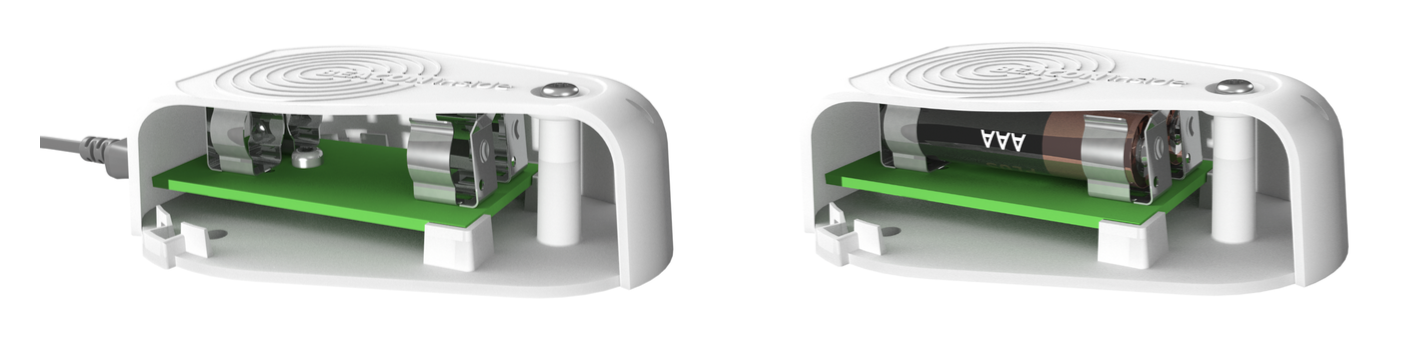
\includegraphics[width=0.6\textwidth]{figures/BEACONinside_beacons}
\caption{3D slice of used beacons from BEACONinside. Source:~\cite{binside:ds}}
\label{fig:bi:beacons}
\end{figure}

The beacons' size is 5.8~cm~x 7,96~cm~x 2.25~cm.
The hardware can either be powered with two AAA~batteries two provide a lifespan of approx.\ one year, or with an external power supply over micro usb~\cite{binside:ds}.

BEACONinside's beacons can be configured with standard \acs{BLE} tools, like capable smartphone apps.
Such an App establishes a \acs{BLE} connection to the beacon.
Each of the following configurable values can be accesed with a specific key.
To configure the beacons we used an iOS app called \textit{LightBlue --- Bluetooth Low Energy}\footnote{Link to the LightBlue App in the iOS AppStore (last access: 18.02.2015) \url{https://itunes.apple.com/de/app/lightblue-bluetooth-low-energy/id557428110}} from a company named \textit{Punch Through Design LLC.}, reccomended by BEACONinside.\\
\newline
Configurable values~\cite{binside:ds}:
\begin{itemize}
  \item \textbf{\texttt{proximityUUID}:} e.g.\ \texttt{F0018B9B-7509-4C31-A905-1A27D39C003C}
  \item \textbf{\texttt{major}:} A value between 1 -- 65535
  \item \textbf{\texttt{minor}:} A value between 1 -- 65535
  \item \textbf{\texttt{Tx-power level}:} It defines the power which is being used to send the beacons advertisement packets, resp.\ the signals. It can either be 0~dBm (default) which is the maximum power, -6~dBm or -23~dBm wich is the minimum power level.
  \item \textbf{\texttt{Advertising interval}:} Defines the time interval (100~ms -- 10s) in which advertisements are being send. The default time interval is 400~ms, configurable in steps of 625~us.
  \item \textbf{\texttt{Calibration value}:} To estimate the distance of the receiving device to the beacon a calibration step is necessary. The measured \acs{RSS} in a distance of one~meter needs to send be send by the beacon with every advertisement. This value can be configured for each \texttt{Tx-power level}. The default is 65~dBm for the 0~dBm power level. It needs to be set as the 2' complement.
  \item \textbf{\texttt{Passkey}:} To write a property the (6 decimal digit) passkey must be supplied. The default value is \texttt{555555}.
\end{itemize}

It is also possible to reboot the device be setting a specific value, which is being necessary to load the new values after changing its configuration, and to reset it to factory defaults.\\
\newline
There are also read-only properties which provide data about the device and its state~\cite{binside:ds}:
\begin{itemize}
  \item \textbf{\texttt{Device Name}:} The beacon's name consiting of \texttt{BEACON} and the latter three bytes of its \acs{MAC} adress.
  \item \textbf{\texttt{Model Number}}
  \item \textbf{\texttt{Serial Number}}
  \item \textbf{\texttt{Hardware Revision Number}}
  \item \textbf{\texttt{Software Revision Number}}
  \item \textbf{\texttt{Manufacturer Name}}
  \item \textbf{\texttt{Battery Level}:} In percent.
  \item \textbf{\texttt{Temperature}:} The hardwares temperature in degrees Celsius.
\end{itemize}

\paragraph{Deployment and Calibration}
As mentionend before, the \acs{BLE} signals quality is heavily influenced by physical materials due to the fact that \acs{BLE} uses the 2.4~GHz frequency.
Especially, water which is a main part of the human body, attenuates the signal~\cite{apple:getting_started}.
Thus, the beacons need to be carefully deployed in its environment.
Ideally, they should be deployed in a manner, that most often the line between beacon and receiver is unobstructed.
There should also be enough space around the beacon, that its signal can spread out.
By deploying them carefully, the signal's attenuation, and other effects like multi-path fading and shadowing can be reduced~\cite{apple:getting_started, IEEE:survey_wireless_indoor_pos}.

The next step is the calibration step. To be able to estimate the distance between smartphone and beacon a reference value is needed. The reference value as mentionend before is the measured \acs{RSS} in a distance of 1~meter to the beacon. The calibration value is being configured on the beacon itself, which includes it in the send advertisement together with its id.

According to Apple, the smartphone needs to be positioned in 1~meter distance to the beacon in portrait mode, with the device's top half uncovered.
Than the \acs{RSS} values where collected for at least 10~seconds.
Meanwhile, the user should slowly move the device on a approx.\ 30~cm line in front of the beacon, by maintaining distance and orientation.
After collecting the values, the average value is being calculated and configured on the beacon~\cite{apple:getting_started}.
It is advisable, to double check the device's estimated distance after setting the calibration value.
Due to the above mentionend problems, this must of course be repeated for every beacon.

\section{iOS 8.1 --- API}
After imparting, what beacons are and how they work, we are focussing in this section on the receivers side --- especially on the \acs{API} provided of Apple's iOS 8.1 platform.
The \textit{Core Location} framework, provides in terms of iBeacons two functionalities called \textit{region monitoring} and \textit{beacon ranging} \cite{apple:ios_doc_cl}.

\paragraph{Region monitoring} As the name already implies, the operating system monitors a spezified region and notifies the application when the user did enter or left the region.
This functionality is not restricted to regions that are marked by a beacon. It already existed long before and monitors also circular regions specified by a distance around a global position in longitude and latitude.
The operating system monitors the specified regions also if the application itself is no running to wake it up if the user enters or leaves a region.

\paragraph{Proximity to a Beacon} To continuously estimate the proximity to a beacon, ranging must be used.
Therefor a \texttt{CLBeaconRegion} needs to be specified.
The \texttt{CLBeaconRegion} object requires at least the beacons' \texttt{proximityUUID}.
It is also possible to specifiy a more specific beacon group by adding the groups  \texttt{major} identifier.
By passing additionally the \texttt{minor} identifier too, the framework just ranges for one specific beacon~\cite{apple:ios_doc_cl}.

After starting the ranging, the framework starts to notify the before specified \texttt{delegate} in a countinously manner after it received the first advertisement of a beacon it is supposed to range for.
This means that the framework does not call the delegate until it received the first matching beacon advertisement.
After the first call it continuouly calls the delegate approximatly every second regardless of wheather it actually received a beacons' advertisment or not.

The delegate gets passed an array of \texttt{CLBeacon} objects.
Each of it represents one beacon.
Figure~\ref{fig:beaconExampleData} shows two example data sets, which the \texttt{CLLocationManager} passed to its delegate. Each data set contains four \texttt{CLBeacon} objects. The table's last entry represents a beacon, which was out of range.

A \texttt{CLBeacon} object contains on one side the beacon's identifiers, as described in section~\ref{sec:beacon}.
On the other side it contains the \textbf{\texttt{rssi}} property which stores the \acl{RSS} measured in dBm.
It expresses how strong the received signal is.
As mentioned before, the beacons' advertisement time interval can be specified.
Remember the beacons from BEACONinside we used are sending their advertisement per default every 400~ms.
The framework itself does stick to its approx.\ 1~second time interval.
It collects all received advertisements and calculates the average since the last reported \texttt{rssi} value~\cite{video}.
If a beacon's signal was received before but not in this time intervall the value is 0.

The \textbf{\texttt{proximity}} property's value expresses the relative distance to a beacon. It can either be \texttt{unknown = 0}, \texttt{immediate = 1}, \texttt{near = 2} or \texttt{far = 3}.
\texttt{unknown} means that the proximity could not be detected. One reason could be, that the ranging just started and could not collect enough advertisements. \texttt{immediate} ``represents a high level of confidence that the device is physically very close to the beacon''~\cite{apple:getting_started}.
The \texttt{near} state is reported, if the user is in approx.\ 1 -- 3~m proximity to the beacon. Thus \texttt{immediate} is reported if the user is closer than approx.\ 1~m.
\texttt{far} is being reported if the ``beacon device can be detected but the confidence in the accuracy is too low to determine either Near or Immediate''~\cite{apple:getting_started}. Hence, the estimated distance is larger than approx.\ 3~m.

%The \acs{RSS} is also being used to calculate the \texttt{CLBeacon} object's \textbf{\texttt{accuracy}} property.
The object's \textbf{\texttt{accuracy}} property actually expresses the proximity to a beacon in meters, but Apple describes the property in its iOS~8.1 documentation as follows:
\begin{quote}
  ``The accuracy of the proximity value, measured in meters from the beacon.
  [\dots]
  Indicates the one sigma horizontal accuracy in meters. Use this property to differentiate between beacons with the same proximity value. Do not use it to identify a precise location for the beacon. Accuracy values may fluctuate due to RF interference.''\cite{apple:ios_doc_cl}
\end{quote}
Thus, we did first interprete this description as the error of the \texttt{proximity} property's value measured in meters. But this makes of course not much sense, because the \texttt{proximity} value stores a relative value which already implies that the user's proximity to the beacon is in a certain range.\cite{videos}

According to \cite{wang:bt_pos}, the distance $d$, between an iBeacon and a smartphone, which depends on the \acl{RSS}, can be calculated with the formula $d = 10^{-\frac{RSSI + A}{10 * n}}$, where $A$ is the \acs{RSSI} value at a distance of $1m$ and the environmental constant $n$.
To proof our assumtion, that the \texttt{accuracy} value is actually the distance, we did some test measaruments and compared them with our own calculations.
Therefor we measured the \acs{RSS} for certain reference distances and stored the associated \texttt{accuracy} values.
The measurements where taken outdoor with \ac{LOS} between beacon and smartphone, to have the signals quality as less imacted by pysical materials as possible.
After collecting 60 measurements for each reference distance we sorted the data set according their \texttt{rssi} values and calculated the average of the \texttt{accuracy} values per \texttt{rssi}.
Afterwards, we used the above mentioned formular to calculate the distance for each measured \texttt{rssi} value.
During the measurements, the beacon's calibration value was set to 65dBm, thus $A = 65dBm$. To approximate the \texttt{CLBeacon} object's \texttt{accuracy} measurements best, an environmental factor of $n = 2.1$ was used, which is similar to the one used by Wang et al \cite{wang:bt_pos}.
Figure~\ref{fig:eval_accuracy_vs_distance} illustrates the result and the fact, that the \texttt{CLBeacon} object's \texttt{accuracy} property's value is the estimated distance between beacon and smartphone.

\begin{figure}
  \begin{tikzpicture}
    \begin{axis}[width=0.9\textwidth, height=0.45\textheight,
        xlabel={\texttt{rssi} (dBm)},
        ylabel={\texttt{accuracy} (m)},
        legend pos=north west,
        legend entries={measurement, avg.\ \texttt{accuracy} per \texttt{rssi}, $d = 10^{-\frac{rssi + 65}{10 * 2.1}}$},
      grid = major,
      x dir=reverse, ymin=0]
      \addplot [only marks, mark=x] table[col sep=semicolon, x=rssi, y=accuracy] {csv/2014-10-15_hoehenweg/all.csv};
      \addplot [red, mark=triangle*, mark size=3pt] table[col sep=semicolon, x=rssi, y=avgAccuracy] {csv/2014-10-15_hoehenweg/all_avg_accuracy_per_rssi.csv};
      \addplot[blue, domain=-55:-95, samples=100]{10^(-(x+65)/(10*2.1))};
  \end{axis}
\end{tikzpicture}
\caption{Dependency on \texttt{CLBeacon} object's \texttt{rssi} and \texttt{accuracy} properties \cite{apple:ios_doc_cl, wang:bt_pos, kotanen:exp_local_pos_bt}.}
\label{fig:eval_accuracy_vs_distance}
\end{figure}

%The estimated distance in meters between the beacon and the device. If beacon's signal was received before but not in this time intervall the value is -1.

% TODO: dBm is a logarithmic unit. Explain dB. can be seen in Figure

\begin{figure}
\begin{tabular}{*{7}{c}}
time & proximityUUID & major & minor & proximity & accuracy & rssi \\
\hline
1.0400 & F0018B9B-\dots-1A27D39C003C & 21500 & 48945 & 2 & 1.2915 & -67\\
1.0400 & F0018B9B-\dots-1A27D39C003C & 39821 & 56686 & 2 & 5.9948 & -79\\
1.0400 & F0018B9B-\dots-1A27D39C003C & 41738 & 1201 & 3 & 6.8129 & -80\\
1.0400 & F0018B9B-\dots-1A27D39C003C & 38722 & 6270 & 3 & 7.7426 & -81\\
 & & & & & & \\
2.0387 & F0018B9B-\dots-1A27D39C003C & 21500 & 48945 & 2 & 1.4452 & -68\\
2.0387 & F0018B9B-\dots-1A27D39C003C & 39821 & 56686 & 3 & 5.5235 & -78\\
2.0387 & F0018B9B-\dots-1A27D39C003C & 41738 & 31201 & 3 & 6.8129 & -80\\
2.0387 & F0018B9B-\dots-1A27D39C003C & 38722 & 6270 & 0 & -1 & 0\\
\end{tabular}
\caption{Recorded beacon example data. Each row represents a \texttt{CLBeacon} object. The table contains two successive datasets.}
\label{fig:beaconExampleData}
\end{figure}


% Wenn es genauigkeit wäre müsste es an den Übergängen von klein zu groß ja auch einen sichtbaren unterschied geben

\section{Evaluation}
After explaining how beacon advertismements can be received with Apple's mobile operating system and which data can be accessed, we are evaluating the data, especially the \texttt{accuracy} properties values, which is the one being used for the later discussed algorithm.
First, we are focussing on the distance estimations quality in terms of its error under different environmental curicumstances.
Afterwards, we present the result of our experiment of using pure multilateration to implement a simple localization algorithm.

\paragraph{Distance estimation}
%As mentionend before, the signals are heavily influenced by physical materials, which also has an impact on the estimated distance.
%Thus, obstacles between sender and receiver are impacting the distance estimation and as well the environments construction.
%But physical materials are not the only reason.
%The device's relative attitude to the beacon

The measured distance provided by the \texttt{CLBeacon} object's \texttt{accuracy} property varies in dynamic but also in a steady and unobstructed environment.

The first reason is, that the \texttt{rssi} values are not directly mapped to the \texttt{accuracy} values.
Apple's \texttt{CoreLocation} framework seems to apply a filter to estimate the distance.
We recorded the \texttt{CLBeacon} object's properties over time at a fixed position with a distance of $2m$ to the beacon.
We directly began recording the data after positioning the phone.
Figure~\ref{fig:beacon_eval_accuracy-rssi} illustrates the behaviour, by showing the \texttt{rssi} values and their corresponding \texttt{accuracy} values over time.
The graph shows, that the \texttt{accuracy} values slowly converge against the actual distance of $2m$. It also shows, that outliers in the \texttt{rssi} property do not have a direct impact on the estimated distance.\newline

\begin{figure}
  \begin{tikzpicture}
    \begin{axis}[width=0.9\textwidth, height=0.45\textheight,
      xlabel={Time (sec)},
      axis y line*=left,
      ylabel={\texttt{accuracy} (m)},
        legend pos=south west,
      legend entries={\texttt{accuracy}, ref.\ distance}]
      \addplot [blue, mark=x] table[col sep=semicolon, x=time, y=accuracy] {csv/2014-10-27_htwg_f007/04_2m.csv};
      %\addlegendentry{accuracy}
      %\addplot [blue, only marks, mark=x] table[col sep=semicolon, x=time, y=accuracy] {csv/2014-10-27_htwg_f007/06_4m.csv};
      \addplot [black, dashed, domain=0:59, samples=2]{2};\label{distance}
      %\addlegendentry{distance}
      %\addplot [blue, dashed, domain=0:59, samples=2]{4};
  \end{axis}
  \pgfplotsset{every axis y label/.append style={rotate=180, yshift=15cm}}
  \begin{axis}[width=0.9\textwidth, height=0.45\textheight,
    axis y line*=right,
    ylabel={\texttt{rssi} (dBm)},
    hide x axis,
    y dir=reverse,
    legend entries={\texttt{rssi}}]
    %\addlegendimage{/pgfplots/refstyle=distance}\addlegendentry{RSSI}
    \addplot [red, mark=*] table[col sep=semicolon, x=time, y=rssi] {csv/2014-10-27_htwg_f007/04_2m.csv};
    %\addplot [blue, only marks, mark=x] table[col sep=semicolon, x=time, y=rssi] {csv/2014-10-27_htwg_f007/06_4m.csv};
  \end{axis}
\end{tikzpicture}
\caption {Dependency of the \texttt{CLBeacon} object's \texttt{accuracy} and \texttt{rssi} property over time with an actual distance of $2m$.}
\label{fig:beacon_eval_accuracy-rssi}
\end{figure}

The second reason is the device's attitude relative to the beacon, but also due to obstacles between the beacon and smartphone.
Figure~\ref{fig:beacon_eval_situations} shows the impact on the estimated distance and the \acs{RSS} in different typical situations.
In each situation the distance between the two devices was $1m$. The measurements where taken indoor. The values shown in figure~\ref{fig:beacon_eval_situations} are average values. For each value 60 --- 100 values where recorded.

\textbf{Situations:}
\begin{itemize}
  \item \emph{(1)} Horizontal iPhone in front of vertical beacon with \acs{LOS}.
  \item \emph{(2)} Horizontal iPhone sideways with \acs{LOS} to vertical beacon.
  \item \emph{(3)} Horizontal iPhone below vertical beacon with \acs{LOS} (Distance 1m, 45 degree below beacon).
  \item \emph{(4)} Vertical iPhone in front of vertical beacon with \acs{LOS}.
  \item \emph{(5)} Horizontal iPhone in front of horizontal beacon with \acs{LOS}.
  \item \emph{(6)} Horizontal iPhone in front of vertical Beacon with person in between.
  \item \emph{(7)} Horizontal backwards turned iPhone in front of vertical Beacon with \acs{LOS}.
  \item \emph{(8)} Horizontal backwards turned iPhone in front of vertical Beacon with person in between.
  \item \emph{(9)} Horizontal iPhone in front of vertical Beacon with 30 cm ferro concrete wall in between.
\end{itemize}

Situation 1, 2, 5 and 7 show, that if the iPhone is horizontal in front or sideways of the vertical beacon vertical with \acs{LOS} the \acs{RSS} attenuation is least.
If the signals are received by the phone with a different angle, shown in situation 3 and 4, the attenuation increases.
A human body between the phone and beacon (situation 6 and 8 has a much higher imact. The estimated distance increases in this example aprox.\ 3 meters.
A ferro concrete 30 cm wall (situation 9) increases the impact again. The phone estimates a distance of 9 meters instead of 1 meter.

The scenarios are very common if a person travels trough a building or room, especially if multiple beacons are deployed.
The problem is, that it is not distinguisable if a estimated distance is being impacted by a wall or a person, with out knowing its own exact position and the positions of all obstacles.\newline

\begin{figure}
 \subfloat[Average accuracy in different situations]{
  \begin{tikzpicture}
    \begin{axis}[width=0.45\textwidth, height=0.4\textheight,
        title={Average accuracy in different situations},
        xlabel={Situation},
        ylabel={Accuracy (m)},
        xtick=data,
      grid = major]
      \addplot [only marks, mark=*] table[col sep=semicolon, x=measurement, y=accuracy] {csv/2014-10-27_htwg_fk034_angles/all_avg.csv};
  \end{axis}
\end{tikzpicture}
}
\subfloat[Average \acs{RSSI} in different situations]{
  \begin{tikzpicture}
    \begin{axis}[width=0.45\textwidth, height=0.4\textheight,
        title={Average \acs{RSSI} in different situations},
        xlabel={Situation},
        ylabel={RSSI (dBm)},
        y dir=reverse,
        xtick=data,
      grid = major]
      \addplot [only marks, mark=*] table[col sep=semicolon, x=measurement, y=rssi] {csv/2014-10-27_htwg_fk034_angles/all_avg.csv};
  \end{axis}
\end{tikzpicture}
}
\caption {Measurement curicumstances: The measurements where taken indoor (HTWG Konstanz FK034) with a distance of 1 m between iBeacon and smartphone. For each situation 60-100 values where measured.\\
}
\label{fig:beacon_eval_situations}
\end{figure}


To depict that the accuracy also varies in steady unobstructed environments with \acs{LOS}, we recorded the \texttt{accuracy} values for different reference distances in different environements.
We recorded for each reference distance 60 values.
We recalibrated the used beacon for each environement.

Figure~\ref{fig:beacon_dispersion_outdoor} illustrates the collected \texttt{accuracy} values measured at 1, 2, \ldots, 5, 10, \ldots, 30 meters distance to the beacon. The measurements where taken outdoor with \acl{LOS} between the two devices.
The graph shows, that the average \texttt{accuracy} measured at 1, 2, 3 and 4 meters distance is very close to the actual distance.
It also shows, that the values disperion for these distances is very low.
After 5 and more meters distance, the dispersion increases and sways between small and huge dispersion, thus it is not correlated to the reference distance.
Compared to the measurements of 1, \ldots, 4 meters the error increases and sways.
As mentionend before the beacons manufacturer claims a maximum range of 40 meters, which is true.
We could range the beacon in this scenario up to a distance of 42 meters.

We repeated the exact same experiment in an indoor environement, figure~\ref{fig:beacon_dispersion_f-cellar} depicts the measurement results.
Also in this case the average \texttt{accuracy} comes very close to the actual distance with a very low disperion for the first 4 distances.
At 5 meters the disperion and error increases and sways, too.
Interestingly, the dispersion starts to decreases from 10 --- 30 meters from a very high to a much smaller value.
At the same time the error grows because due to the \acs{RSS} the smartphone estimates a very low distance whereas the actual distance is very high.
The assumend reason is the test environements construction form. The measurments where recorded in a straight long but slim corridor in a cellar. There are multiple doors, made of steel, on both sides of the wall that maybe caused reflections.

The depicted measurements in figure~\ref{fig:beacon_dispersion_f007} are recorded in a approx.\ 15 meter long and 8--11 meters wide lecture hall.
It shows, that also the first few meters on average are matching best, but it also depicts, that the sometimes huge differences in the distance estimation recorded at the same position.

As mentioned in chapter~\ref{PF-Foundation??}, it is necessary to know the uncertainties of a measurement to implement a particle filter.
Figure~\ref{fig:beacon_eval_ndf} depicts the parameters to model the distance estimations' uncertainties with a \acs{NDF}.
Therefor, the data of figure~\ref{fig:beacon_dispersion_outdoor} and \ref{fig:beacon_dispersion_f007} was being used.
The two dashed straight lines show the linear function that approximates the standard deviation $\sigma$ depending on the mean value $\mu$ best.\\ \newline

\begin{figure}
  \subfloat[Outdoor]{
  \begin{tikzpicture}
    \begin{axis}[trim axis left, trim axis right, width=0.45\textwidth, height=0.45\textheight,
        xlabel={Reference distance (m)},
        ylabel={\texttt{accuracy} (m)},
        legend pos=north west,
        legend entries={accuracy, avg. accuracy},
        grid = major]
      \addplot [only marks, mark=x] table[col sep=semicolon, x=proximityRef, y=accuracy] {csv/2014-10-15_hoehenweg/all.csv};
      \addplot [red, only marks, mark=triangle*, mark size=3pt] table[col sep=semicolon, x=proximityRef, y=avgAccuracy] {csv/2014-10-15_hoehenweg/avg_all.csv};
      \addplot [black, dashed, domain=0:30, samples=2]{x};
  \end{axis}
\end{tikzpicture}
\label{fig:beacon_dispersion_outdoor}

}
\subfloat[HTWG-KN cellar F-Building]{
  \begin{tikzpicture}
    \begin{axis}[width=0.45\textwidth, height=0.45\textheight,
        xlabel={Reference distance (m)},
        ylabel={\texttt{accuracy} (m)},
        legend pos=north west,
        legend entries={accuracy, avg. accuracy},
        grid = major]
      \addplot [only marks, mark=x] table[col sep=semicolon, x=proximityRef, y=accuracy] {csv/2014-10-15_htwg_keller_f/all.csv};
      \addplot [red, only marks, mark=triangle*, mark size=3pt] table[col sep=semicolon, x=proximityRef, y=avgAccuracy] {csv/2014-10-15_htwg_keller_f/all_avg_accuracy_per_proximity.csv};
      \addplot [black, dashed, domain=0:30, samples=2]{x};
  \end{axis}
\end{tikzpicture}
\label{fig:beacon_dispersion_f-cellar}
}

\subfloat[HTWG-KN F007]{
\begin{tikzpicture}
    \begin{axis}[width=0.45\textwidth, height=0.45\textheight,
        %title={Dispersion of CLBeacon's accuracy property.},
        xlabel={Reference distance (m)},
        ylabel={\texttt{accuracy} (m)},
        legend pos=north west,
        legend entries={accuracy, avg. accuracy},
        grid = major]
      \addplot [only marks, mark=x] table[col sep=semicolon, x=proximityRef, y=accuracy] {csv/2014-10-27_htwg_f007/all.csv};
      \addplot [red, only marks, mark=triangle*, mark size=3pt] table[col sep=semicolon, x=proximityRef, y=avgAccuracy] {csv/2014-10-27_htwg_f007/all_avg_accuracy_per_proximity.csv};
      \addplot [black, dashed, domain=0:14.5, samples=2]{x};
  \end{axis}
\end{tikzpicture}
\label{fig:beacon_dispersion_f007}
}
\caption {Accuracy dispersion plot. The measurements with \ac{LOS} between beacon and smartphone. For each reference distance 60 accuracy values where measured.}
\label{fig:beacon_dispersion}
\end{figure}



\begin{figure}
  \begin{tikzpicture}
    \begin{axis}[trim axis left, trim axis right, width=0.9\textwidth, height=0.45\textheight,
        %title={Normal Distribution Function parameters},
        xlabel={Mean $\mu$ (m)},
        ylabel={Standard deviation $\sigma$ (m)},
        legend pos=south east,
        legend entries={outdoor, $f(\mu)=0.3286 \cdot \mu + 0.8379$, indoor (HTWG-KN F007), $f(\mu)=0.3131 \cdot \mu + 0.0051$},
      grid = major]
      \addplot [red, mark=*] table[col sep=semicolon, x=mu_distance, y=sigma_distance] {csv/2014-10-15_hoehenweg/ndf_parameters.csv};
      \addplot [red, dashed, domain=0:30, samples=2]{0.3286*x+0.8379};
      \addplot [blue, mark=*] table[col sep=semicolon, x=mu_distance, y=sigma_distance] {csv/2014-10-27_htwg_f007/ndf_parameters.csv};
      \addplot [blue, dashed, domain=0:30, samples=2]{0.3131*x+0.0051};
  \end{axis}
\end{tikzpicture}
\caption{Depicts the uncertainties of the distance estimation modeled with a normal distribution function.}
\label{fig:beacon_eval_ndf}
\end{figure}

The experiment's result show, that the distance estimation not just depend on the beacons calibration, it also depends on the buildings construction form, the phones realtive attitude to the beacon and the obstacles in between.
It also points out, that the \texttt{CLBeacon}'s \texttt{accuracy} resp.\ the estimated distance comes very close to the actual distance up to 4, 5 meters with \acs{LOS}.
Larger distances cause a much higher dispersion and also a larger error.
Physical material like humans and walls do cause attenuation, which results in a larger distance as it actually is.
Thus, the estimated distances are very unreliable due to the fact, that the validity cannot be proofed, without knowing the receivers exact position and the properties of all other influencing factors.

\paragraph{Multilateration}
After evaluating the distance estimation's quality of one beacon, we decided to deploy some beacons in a lecture hall to get a better feeling of how good the distance estimation actually works.
On one side the goal was to visualize the estimated distances on a map to proof their plausability, and on the other side to test if indoor self-localization with smartphones is possible by just using iBeacons without integrating additional sensor data.

Lateration is a method to estimate a position by estimating the distance to the sender of a wireless signal by using the \acs{RSS}.
Thus, multilateration means, to estimate the position by using the distances to several senders.
Angulation (often named Triangulation) is a similar method. Instead of estimating the distance to a sender it uses the angle resp. the direction where the signal comes from relative to the receiver.
Trilateration resp. -angulation means that three senders are being used to estimate the position.

The receivers position with just one sender is somewhere on a circle around the sender with the estimated distance as radius of the circle.
By using two senders $s_1$ and $s_2$, the two circles around the senders can have zero, one or two intersections, if the position of $s_1 \neq s_2$. Thus, the receivers position must be at one of the circles' intersections.
By adding a third sender $s_3$ the three circles have either no or exactly one common intersection point, which is the reveivers position.
This applies also to more than three senders.

To be able to use our implementation with variable sender count, we use the \emph{Least Square} method to determine the receivers position. Another advantage is, that the least square method can also estimate a position if no common intersection point exists, e.g. if just two of four circles intersect with each.

For our experiment we used the same lecture hall as before.
There, we positioned four beacons.
Then we used our iPhone~5S test device recoded the received beacon identifieres and the by the \texttt{CoreLocation} estimated distances (\texttt{accuracy} values), during our test walk on a defined path.
To visualize the estimated distances to the beacons and the estimated position resp. the walked path we wrote a small programm in Python.
Figure~\ref{fig:beacon_eval_multilat} shows four screenshots of the programs output.
Each of it shows a map, which shows the lecture halls walls in grey.
The white space in the hall is free space.
The filled small blue circles next to the walls are the four beacons.
The big blue cirles are the circles around the beacon where the radius equals the estimated distance to the beacon.
We did one walk on the green tetragon beginning at the bottom right corner in counter clockwise direction, with holding the test device in front of us. The beacons where positioned in approximately the same hight.
The red line shows the path estimated by our multilateration implementation.

Screenshot a shows, that the estimated distance sometimes is completely wrong, as the one to the beacon in the top-right corner.
It also shows that the estimated position is somewhere several meters outside of the lecture hall.
The second screenshot shows, that the distance to the top-right beacon shrinks, but one to the top-left massively grows. The distances to the other two beacons seem to be plausible.
The third one shows a plausible position. It also shows that in this step the bottom-right beacon's signal was not received.
The last screenshot shows also a more or less plausible position. The distances, except the one to the bottom-left beacon, seem to be plausible.

This experiment shows, that the beacons signals must be heavily influenced, due to the very unreliable distance estimations.
It also shows that pure multilateration method, without filtering the data and without integrating additional data sources, is not sufficient enough for indoor self-localization, because sometimes the positon is several meters outside the room.

\begin{figure}
  \subfloat[]{
    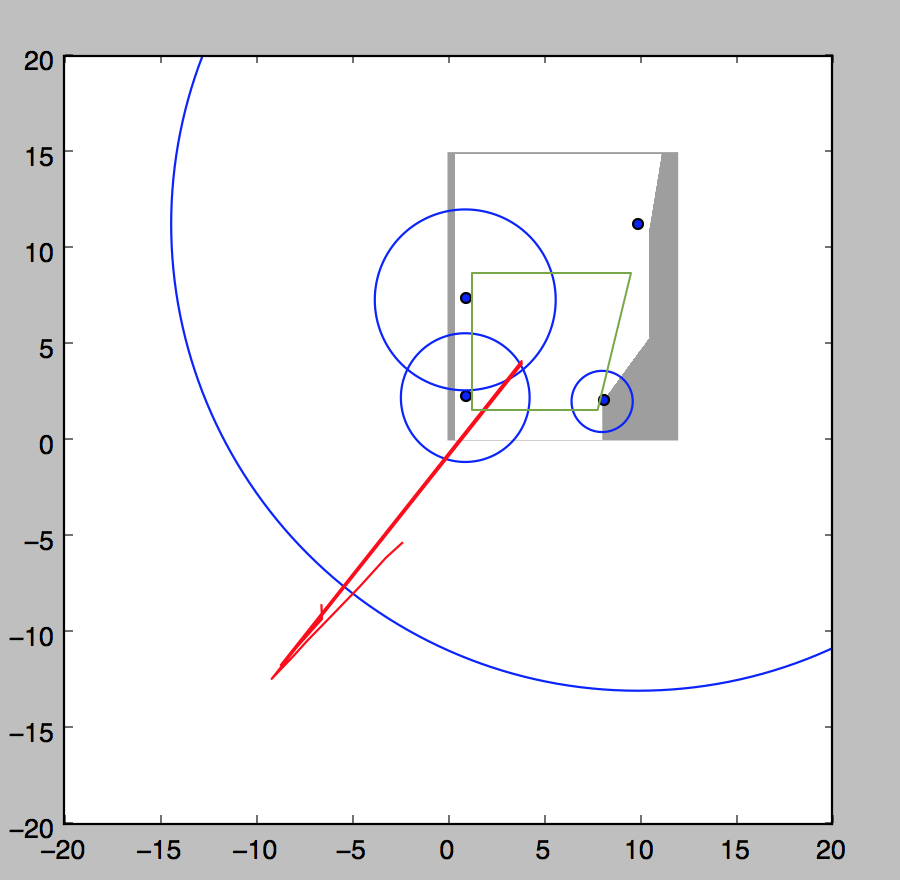
\includegraphics[width=0.45\textwidth]{figures/multilat_1}
  }
  \subfloat[]{
    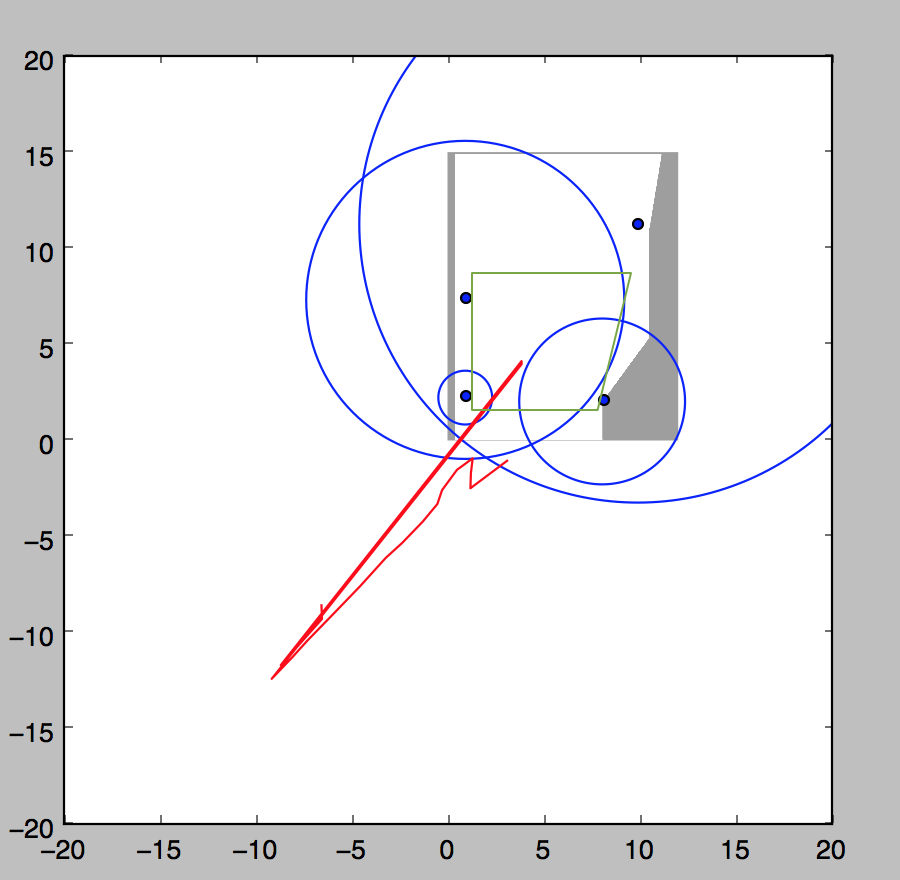
\includegraphics[width=0.45\textwidth]{figures/multilat_2}
  }

  \subfloat[]{
    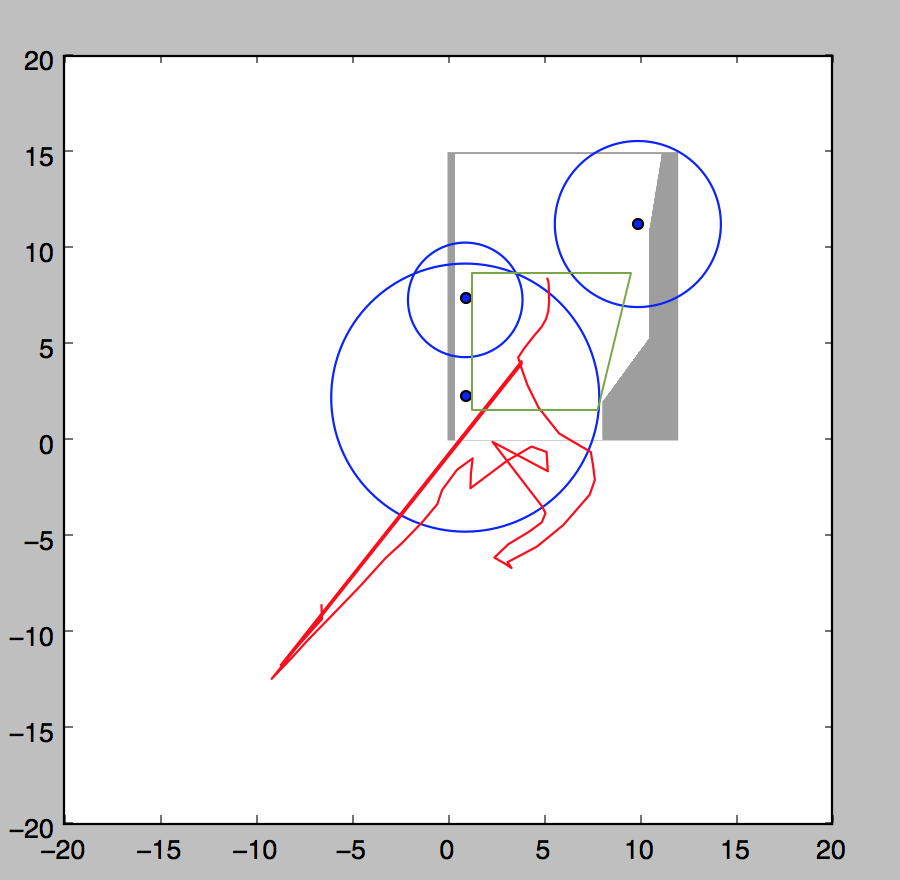
\includegraphics[width=0.45\textwidth]{figures/multilat_3}
  }
  \subfloat[]{
    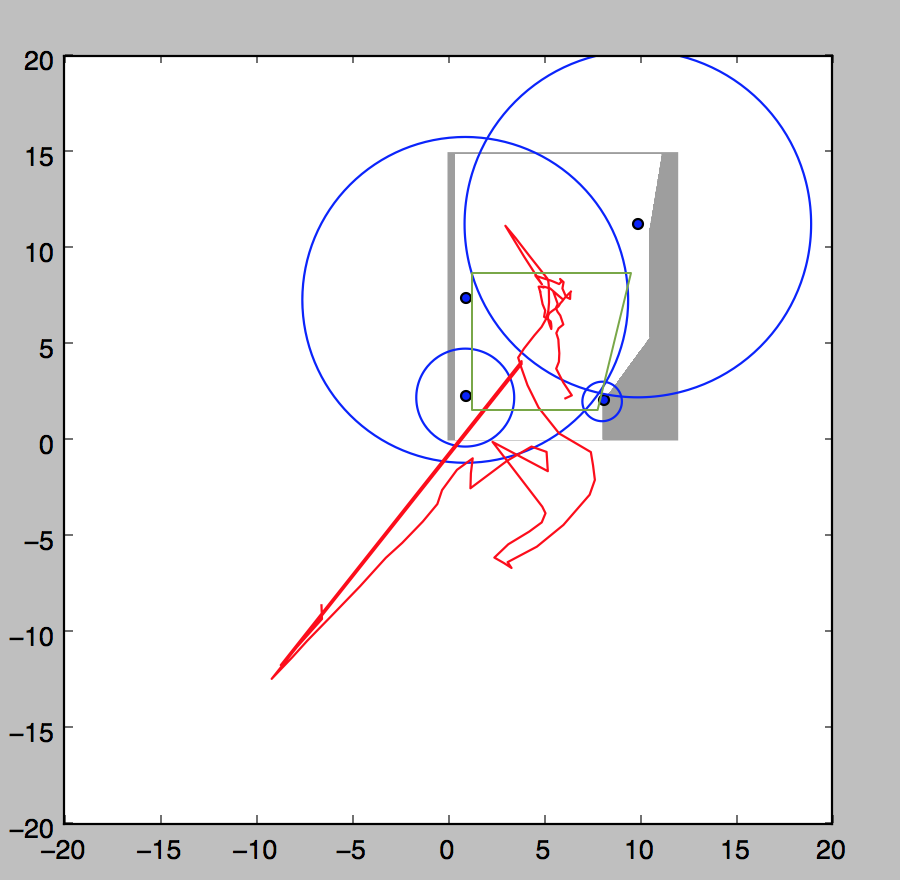
\includegraphics[width=0.45\textwidth]{figures/multilat_4}
  }
  \caption{Screenshots of indoor self-localization experiment using multilateration.}
  \label{fig:beacon_eval_multilat}
\end{figure}


\paragraph{Summary}
To summarize, the beacons' signals reps. the estimated distances are very unreliable, due to the signals influences by physical materials.
Distance estimations for distances larger than 5 meters are often wrong.
Thus, their plausibility should be proofed to weight or filtered them out.
But it is very difficult to check their plausibility in large buildings without knowing the receivers position.
Hence, they can just be ignored.

Another problem are distance estimations, that are less than 5 meters but actually more than 5 meters. These errors can not being detected, without knowing the receivers position and consequently they cannot be ignored.
